\section{Nested-Word Automata and Overview of the Library's Organization}
\label{Se:Nested Word Automata}

WALi-NWA is a library for constructing and querying nested-word automata.  It
is implemented in C++.

\subsection{Definitions}
\label{Se:Def}

\begin{definition}
  \label{De:nested word}

  A \textbf{nested-word} $(w,\leadsto)$ over an alphabet, $\Sigma$, is an
  ordinary word $w$, together with a \textbf{nesting relation} $\leadsto$ of
  length $|w|$.  $\leadsto$ is a collection of edges (over the positions in
  $w$) that do not cross.  A nesting relation of length $l \geq 0$ is a
  subset of $\{-\infty,1,2,\ldots,l\} \times \{1,2,\ldots,l,+\infty\}$ such
  that

  \begin{itemize}
    \item Nesting edges only go forwards: if $i \leadsto j$ then $i < j$.
    \item No two edges share a position: for $1 \leq i \leq l$, $|\{j | i
      \leadsto j \}| \leq 1$ and $|\{ j | j \leadsto i \}| \leq 1$.
    \item Edges do not cross: if $i \leadsto j$ and $i' \leadsto j'$, then
      one cannot have $i < i' \leq j < j'$.
  \end{itemize}

  When $i \leadsto j$ holds, for $1 \leq i \leq l$, $i$ is called a
  \textbf{call} position; if $i \leadsto +\infty$, then $i$ is a
  \textbf{pending call}; otherwise $i$ is a \textbf{matched call}, and the
  unique position $j$ such that $i \leadsto j$ is called its
  \textbf{return-successor}.  Similarly, when $i \leadsto j$ holds, for $1
  \leq j \leq l$, $j$ is a \textbf{return} position; if $-\infty \leadsto j$,
  then $j$ is a \textbf{pending return}; otherwise $j$ is a \textbf{matched
    return}, and the unique position $i$ such that $i \leadsto j$ is called
  its \textbf{call-predecessor}.  A position $1 \leq i \leq l$ that is
  neither a call nor a return is an \textbf{internal} position.

  A \textbf{balanced nested-word} is a nested word that has no pending calls
  or returns.  An \textbf{unbalanced-left nested word} (or
  \textbf{nested-word prefix}) is a nested word that has no pending returns.
  An \textbf{unbalanced-right nested word} (or \textbf{nested-word suffix})
  is a nested word that has no pending calls.

\end{definition}

The library supports unbalanced-left, unbalanced-right, and balanced
nested-words, but has no direct support for general nested words.  For the
effects of boolean operations on the four kinds of nested-words see Figure
\ref{Fig:Ops}.

\begin{figure}[htb]
  \centering
\begin{tabular}{c@{\hspace{1cm}}c}
  \begin{tabular}{|| r || l | l | l | l ||}
\hhline{|t:=====:t|}
    Intersection & B & UL & UR & NW \\
\hhline{||=#=|=|=|=||}
    B & B & B & B & B \\
\hhline{||-||-|-|-|-||}
    UL & B & UL & B & UL \\
 \hhline{||-||-|-|-|-||}
    UR & B & B & UR & UR \\
\hhline{||-||-|-|-|-||}
    NW & B & UL & UR & NW \\
\hhline{|b:=====:b|}
  \end{tabular}
\vspace{1cm} &
  \begin{tabular}{|| r || l | l | l | l ||}
\hhline{|t:=====:t|}
    Concatenation & B & UL & UR & NW \\
\hhline{||=#=|=|=|=||}
    B & B & UL & UR & NW \\
\hhline{||-||-|-|-|-||}
    UL & UL & UL & NW & NW \\
\hhline{||-||-|-|-|-||}
    UR & UR & NW & UR & NW \\
\hhline{||-||-|-|-|-||}
    NW & NW & NW & NW & NW \\
\hhline{|b:=====:b|}
  \end{tabular} \\
\vspace{1cm}
  \begin{tabular}{|| r || l | l | l | l ||}
\hhline{|t:=====:t|}
    Union & B & UL & UR & NW \\
\hhline{||=#=|=|=|=||}
    B & B & UL & UR & NW \\
\hhline{||-||-|-|-|-||}
    UL & UL & UL & NW & NW \\
\hhline{||-||-|-|-|-||}
    UR & UR & NW & UR & NW \\
\hhline{||-||-|-|-|-||}
    NW & NW & NW & NW & NW \\
\hhline{|b:=====:b|}
  \end{tabular} &
  \begin{tabular}{|| r || l | l | l | l ||}
\hhline{|t:=====:t|}
    Operation & B & UL & UR & NW \\
\hhline{||=#=|=|=|=||}
    Star & B & UL & UR & NW \\
\hhline{||-||-|-|-|-||}
    Reverse & B & UR & UL & NW \\
\hhline{||-||-|-|-|-||}
    Complement & UL & UL & UR & NW \\
\hhline{|b:=====:b|}
  \end{tabular} \\
\end{tabular}
  \caption{Table of Operations on Nested Words. Note: B = balanced nested-word, UR = unbalanced-right nested-word, UL = unbalanced-left nested-word, NW = nested-word}
  \label{Fig:Ops}
\end{figure}


\begin{definition}
  \label{De:NWA}

  A \textbf{nested-word automaton} (NWA), $A$, is a tuple of the form $A=(Q,
  \Sigma, Q_0, \delta, Q_f)$, where $Q$ is a finite set of states, $\Sigma$
  is a finite alphabet, $Q_0 \subseteq Q$ is a set of initial states, $Q_f
  \subseteq Q$ is a set of final states, and $\delta$ is a transition
  relation. The transition relation $\delta$ consists of three components,
  $(\delta_i, \delta_c, \delta_r)$, where:

  \begin{itemize}
    \item $\delta_i \subseteq Q \times \Sigma \times Q$ defines the
      transition relation for internal positions.
    
    \item $\delta_c \subseteq Q \times \Sigma \times Q$ defines the
      transition relation for call positions.
    
    \item $\delta_r \subseteq Q \times Q \times \Sigma \times Q$ defines the
      transition relation for return positions.
  \end{itemize}
\end{definition}

Starting from some $q_0 \in Q_0$, an NWA $A$ reads a nested word $nw = (w,v)$
from left to right and performs transitions (possibly non-deterministically)
according to the input symbol and the nesting relation. That is, if $A$ is in
state $q$ when reading input symbol $\sigma$ at position $i$ in $w$, then if
$i$ is an internal or call position, $A$ makes a transition to $q'$ using
$(q,\sigma,q') \in \delta_i$ or $(q,\sigma,q') \in \delta_c$,
respectively. Otherwise, $i$ is a return position. Let $k$ be the
call-predecessor of $i$, and let $q_c$ be the state $A$ was in just before
the transition it made on the $k^{\text{th}}$ symbol; then $A$ uses
$(q,q_c,\sigma,q') \in \delta_r$ to make a transition to $q'$.  If, after
reading $nw$, $A$ is in a state $q \in Q_f$, then $A$ accepts $nw$
\cite{DLT:AM2006}.

To distinguish among the different roles for states in an internal
transition, $(q,\sigma,q')$, we say that $q$ is the source and $q'$ is the
target.  Similarly, to distinguish among the roles for states in a call
transition $(q_c,\sigma,q_e)$, we say that $q_c$ is the call state and $q_e$
is the entry state, and to distinguish among the roles for states in a return
transition, $(q_x,q_c,\sigma,q_r)$, we say that $q_x$ is the exit state,
$q_c$ is the call state, and $q_r$ is the return state.


\subsection{Classes}
\label{Se:Classes}

\begin{description}

\item NWA \nopagebreak

  Models nested-word automata.  This is the main class of the WALi-NWA package.

\item NWS \nopagebreak

  Models a nested-word suffix, i.e., an unbalanced-right nested word.  This
  can also model balanced nested words.

\item NWP \nopagebreak

  Models a nested-word prefix, i.e., an unbalanced-left nested word.  This
  can also model balanced nested words.

\item ClientInfo \nopagebreak

  Additional information that can be attached to NWA states.

\item WeightGen \nopagebreak

  Weight-generation algorithms for the NWA to WPDS conversion and prestar and
  poststar reachability queries.

\item Key \nopagebreak

  A special kind of identifier used for uniquely identifying states and
  symbols.  See \cite{wali}.

\item WPDS \nopagebreak

  Models weighted pushdown systems.  See \cite{wali}.

\item WFA \nopagebreak

  Models weighted finite automata.  See \cite{wali}.

\item ref\_ptr$<$T$>$ \nopagebreak

  A reference counting pointer class.  See \cite{wali}. \\

\end{description}


\subsection{Construction}
\label{Se:Construction}

To construct an NWA, a constructor is invoked that creates either an empty
NWA or a one-state NWA.  Thereafter, method calls are performed
to \begin{inparaenum} \item add or remove states, \item add or remove
  symbols, \item add or remove transitions, \item set the status of certain
  states as initial or final, and \item combine component NWAs (via union,
  intersection, etc). \end{inparaenum}


One complication arises due to stuck states.  A stuck state is a state that
can never be a final state and has no outgoing transitions other than to
itself.  The NWA class supports modeling NWAs with a designated stuck state;
in such an NWA, there may be implicit transitions to this stuck state,
whereas an NWA without a stuck state can hove only explicit transitions.  The
remainder of this document uses ``stuck state'' to refer to this
explicitly-designated stuck state.  This means that in an NWA without a stuck
state there must exist a transition of each kind out of every state (out of
every pair of states for return transitions) for every symbol.  Therefore, we
distinguish between two types of NWAs: type 1 - an NWA with a stuck state,
and type 2 - an NWA without a stuck state.  Each state in an NWA of type 2
must be complete; that is, each state must have outgoing transitions for each
symbol of the alphabet.  Operations that add or remove individual states and
individual transitions would cause state-completeness to be violated, and
hence they are disallowed on NWAs of type 2.  If such an operation is applied
to an NWA of type 2, the operation causes an assertion violation.  In NWAs of
type 1, completeness is implicit: a given state has some number (possibly
zero) of explicit outgoing transitions on some number of symbols; for all
other symbols, for each of the three kinds of transitions, there are implicit
transitions to the stuck state.

\textbf{Important Note: Due to the requirement of the completeness of an NWA
  of type 2, states (except the stuck state), symbols, and transitions can
  only be added to an NWA of type 1.}

NWAs can be created in multiple ways: 
\begin{enumerate}
  \item The basic constructor ( \texttt{NWA()} ) constructs an NWA of type 2
    with no states, symbols, or transitions.  An NWA created in this way
    cannot have states, symbols, or transitions added to it until it has a
    stuck state (which can be added using \texttt{setStuckState}).

  \item If the constructor is supplied with a state ( \texttt{NWA( Key
    stuckSt )} ), it constructs an NWA of type 1 (having stuck state
    \texttt{stuckSt}) with $Q = \{\texttt{stuckSt}\}$, and no symbols or
    transitions.

  \item The copy constructor constructs an NWA of the same type as the NWA
    passed in.
\end{enumerate} 

\noindent
The type of an NWA can be checked (using \texttt{hasStuckState}) or changed
(using \texttt{realizeImplicitTrans}, \texttt{clear} for changing an NWA of
type 1 to an NWA of type 2, or \texttt{setStuckState} for changing an NWA of
type 2 to an NWA of type 1) at any time after its construction. \\

\noindent
The following operations are methods of class NWA:

\begin{description}

  \item \texttt{bool hasStuckState()} \nopagebreak

    Tests whether the NWA is of type 1 (returns \texttt{true}) or type 2
    (returns \texttt{false}).

  \item \texttt{void setStuckState( Key stuckSt )} \nopagebreak

    Allows the user to specify a stuck state, \texttt{stuckSt}, thereby
    making an NWA of type 2 into an NWA of type 1.  The state specified must
    not already exist in the NWA (this guarantees that the stuck state will
    not be final or have any outgoing transitions).  Furthermore, because a
    stuck state already exists in anNWA of type 1, if this method is invoked
    on an NWA of type 1 it triggers an assertion violation.

  \item \texttt{void realizeImplicitTrans()} \nopagebreak

    See Section \ref{Se:Transitions}.  Note: Converts an NWA of type 1 into
    an NWA of type 2 having the same behavior.

  \item \texttt{clear()} \nopagebreak

    Removes all states (including the stuck state if there is one, so the
    resulting NWA will always be of type 2), symbols, and transitions from
    the NWA. \\

\end{description}


The only ways to remove a stuck state from an NWA are
to \begin{inparaenum} \item clear all states, symbols, and transitions from
  the NWA using \texttt{clear}, or \item materialize all implicit transitions
  via \texttt{realizeImplicitTrans} (which changes the type of the NWA to
  type 2), set a new stuck state (which changes the type of the NWA back to
  type 1), and remove the old stuck state (which is no longer the stuck state
  of the NWA).\end{inparaenum}


\subsection{Examples}
\label{Se:Examples}

As an example, consider the nested word automaton $A = (Q_A, \Sigma_A,
{Q_0}_A, \delta_A, F_A)$ where $Q_A = \{Start, Call, Entry, State, Exit,
Return, End, Stuck\}$ (with $Stuck$ set as the stuck state), $\Sigma_A = \{a,
call, b, ret\}$, ${Q_0}_A = \{Start\}$, $F_A = \{End\}$, and \\
$\delta_A = 
\begin{cases} 
\delta_i = \{(Start,a,Call), (Entry,b,State), (State,b,Exit), (Return,a,End)\}, \\
\delta_c = \{(Call,call,Entry)\}, \\ 
\delta_r = \{(Exit,Call,ret,Return)\}, \\ 
\end{cases}$
as seen in Figure \ref{Fig:Example1}.  This NWA is of type 1, since there is
a stuck state, $Stuck$, and some transitions are implicit (in fact, in this
NWA, all transitions to the stuck state are implicit.
 
\begin{figure}[htb]
  \centering
    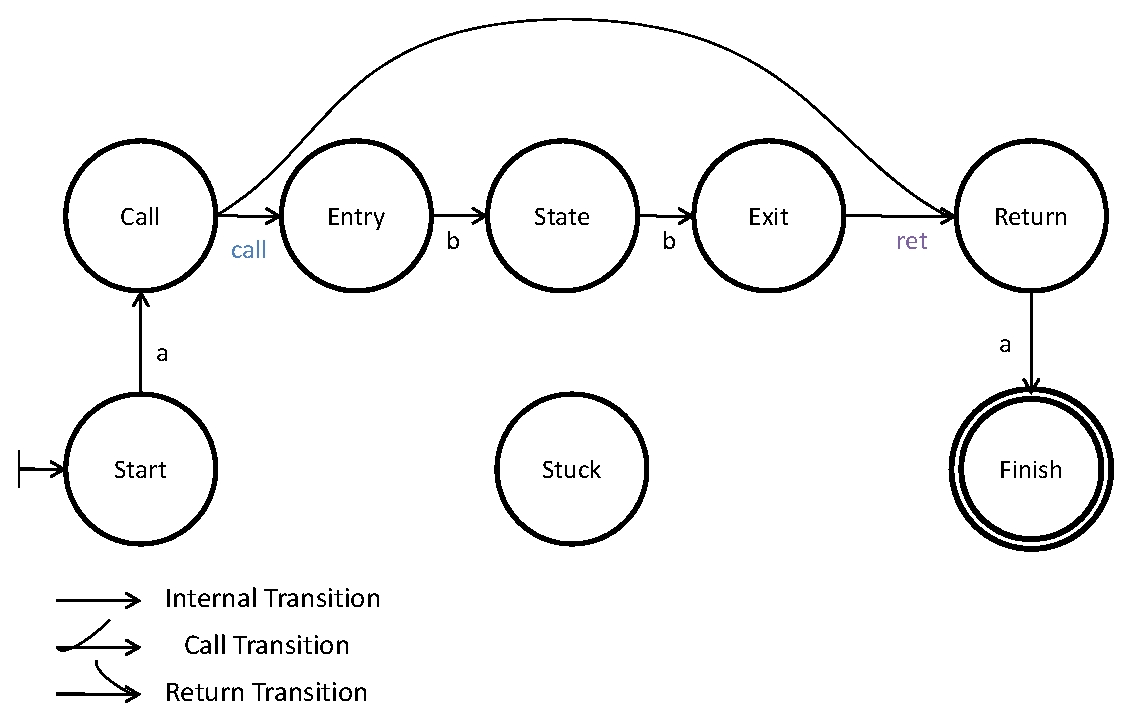
\includegraphics[width=12cm]{Figures/Figure1}
  \caption{An example of an NWA of type 1.}
  \label{Fig:Example1}
\end{figure}


The equivalent nested word automaton of type 2 is shown in Figure
\ref{Fig:Example2}.  Here $Stuck$ is just an ordinary state.  For ease of
reading the lines connecting calls and returns are left out of this diagram.
In reality every return transition to $Stuck$ in Figure \ref{Fig:Example2}
represents as many as 8 return transitions, one for each possible call state,
i.e., the transitions $(Start,Start,a,Stuck)$, $(Start,Call,a,Stuck)$,
$(Start,Entry,a,Stuck)$, $(Start,State,a,Stuck)$, $(Start,Exit,a,Stuck)$,
$(Start,Return,a,Stuck)$, $(Start,Finish,a,Stuck)$, and
$(Start,Stuck,a,Stuck)$ are the return transitions from $Start$ to $Stuck$ on
the symbol $a$.  The number of transitions that each represents appears in
parentheses following the symbol.  Note: If \texttt{realizeImplicitTrans} is
called on the NWA in Figure \ref{Fig:Example1} the result is the NWA in
Figure \ref{Fig:Example2}.

\begin{figure}[htb]
  \centering
    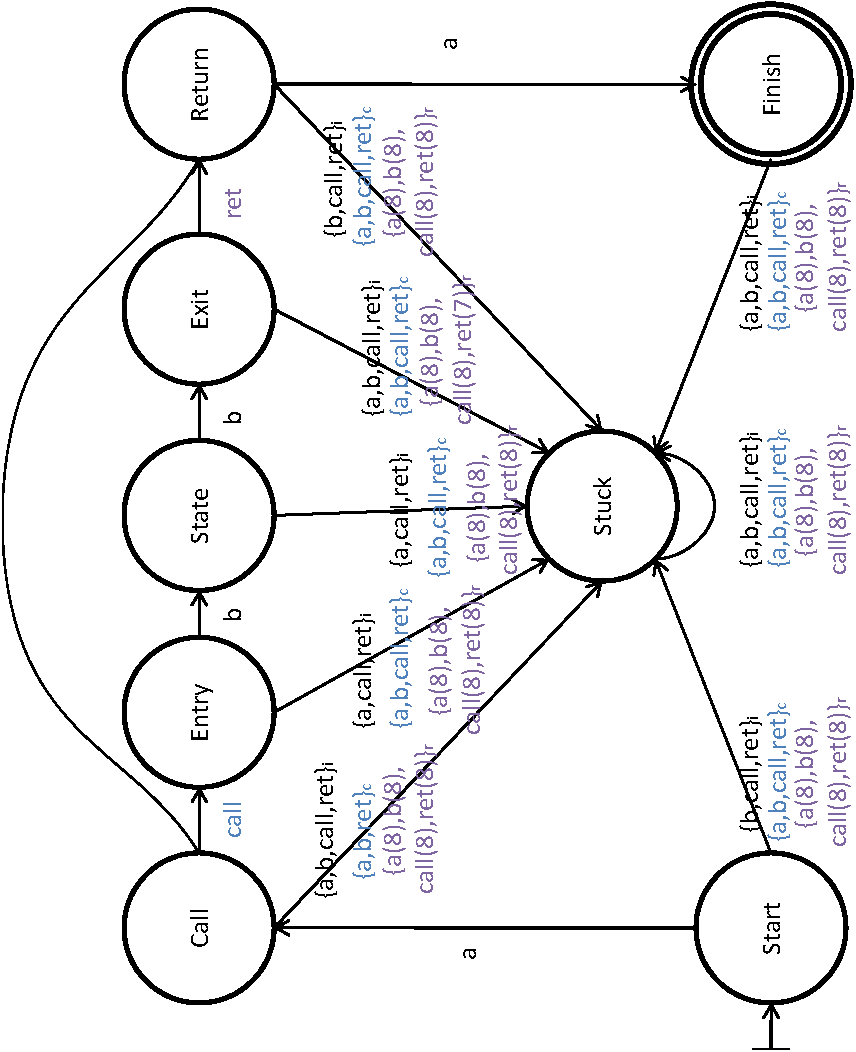
\includegraphics[width=12cm]{Figures/Figure2}
  \caption{An example of an NWA of type 2.  Note: The edge from $Entry$ to
    $Stuck$ labeled $\{a,call,ret\}_i$ is a shorthand for three internal
    transitions in $\delta_i$: $(Entry,a,Stuck)$, $(Entry,call,Stuck)$, and
    $(Entry,ret,Stuck)$.  Similarly, the edges labeled $\{\cdots\}_c$ are
    shorthand for call transitions and the edges labeled $\{\cdots\}_r$ are
    shorthand for return transitions.}
  \label{Fig:Example2}
\end{figure}


